\section{SECH 5}
\subsection{Motivations and Deployment Scenarios}

[ ] arbitrary access for new clients without coordination from server

\subsection{Design}

[ ] server produces an \var{SECHConfig} and corresponding private key for the KEM

[ ] client has to attain \var{SECHConfig} in order to offer SECH 5 in a \var{ClientHello}, can attain over DoH or some other means

[ ] client encapsulates an ephemeral key $k$ using the KEM and public key specified in \var{SECHConfig} producing \var{enc}

[ ] client pads the servername to \var{SECHConfig.servername\_length} producing \var{\paddedServername}

[ ] client encrypts the \var{padded\_servername} with the AEAD specified in SECHConfig, and with key $k$ and a \nonce which is the first 12 octets of the hash of \var{SECH5ClientHelloAAD}, and with \var{SECH5ClientHelloAAD} as AAD, producing \var{sech5\_cipher} which is the concatenation of the encrypted text and the tag $t$

[ ] \var{SECH5ClientHelloAAD} is the \var{ClientHello} but with the portion in which the AEAD cipher (encrypted text and tag) will be placed set to zero, the size and location of this region depends on \var{SECHConfig}

[ ] \var{SECH5ClientHelloAAD} is the \var{ClientHelloOuter} but with the \var{random} and \var{legacy\_session\_id} set to all 0s

[ ] client encodes \var{enc} and \var{sech5\_cipher} in the \var{ClientHello} \var{random} and \var{legacy\_session\_id} fields producing \var{ClientHelloOuter} as depicted in Figure~\ref{fig:sech5-cover}

[ ] the client-facing server attempts to decapsulate \var{enc} with the private key associated with \var{SECHConfig} retrieving $k$, on failure continues with normal TLS 1.3

[ ] the client-facing server computes \var{SECH5ClientHelloAAD} and the \nonce, and then attempts to decrypt $ct$ and authenticate with $t$, on failure continues with normal TLS 1.3

[ ] on success the client-facing server constructs \var{SECH5ClientHelloInner} by replacing $ct$ with $pt$ and setting the \var{extension\_data} of the \var{server\_name} extension to all 0s

[ ] client-facing server forwars \var{SECH5ClientHelloInner} to the backend server

[ ] the backend server proceeds with SECH 5 iff the \var{server\_name} extension has all 0s, otherwise continues with normal TLS 1.3

[ ] the backend server might respond with \var{HRR} or \var{ServerHello}, the \var{HRR} is constructed as normal, but the \var{ServerHello} contains a special \var{sech5\_accept\_confirmation} value in the last 8 octets of the \var{random}


\begin{figure}[htb]
\centering
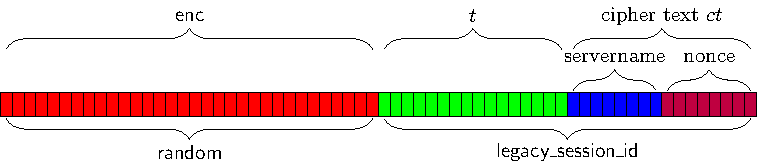
\includegraphics[width=\linewidth]{figure/sech5-cover.pdf}
\captionsetup{width=.8\linewidth} 
\caption[SECH 5 Cover]{}
\label{fig:sech5-cover}
\end{figure}

\subsection{Implementation Notes}